\section{Modelado}
\label{sec:modelado}

Se ajustan dos objetivos sobre las tablas de la fase~3: predecir el nivel del
paralelo y la brecha (\textbf{Objetivo 1}) y medir la relación entre la Gaceta y
la brecha (\textbf{Objetivo 2}). La entrada es la serie horaria (\textbf{4\,321
h}) y el panel diario de \textbf{179 días} con los canales de la Gaceta.

\textbf{Quiebre estructural.} La muestra tiene un solo quiebre: la devaluación
del oficial el \textbf{2026-06-27} (6{,}91 $\rightarrow$ 9{,}73~Bs/USD, $+41\%$).
La ventana de prueba cae íntegra después, así que las métricas miden el período
vigente. El ARIMA se entrena con los 90 días posteriores al quiebre; la regresión
y el HAC usan las 4\,128~h completas.

\subsection{Diseño de validación}

\begin{itemize}
  \item \textbf{Partición temporal fija:} las últimas 168 h, mismo corte para
        todos los modelos.
  \item \textbf{Dos horizontes:} 1 hora y 1 día, con origen móvil y el naïve
        del mismo horizonte como línea base
        \cite{makridakis2020m4}.
  \item \textbf{Métricas:} RMSE y MAE en unidades del target, y su cociente
        frente al naïve.
\end{itemize}

\subsection{Regresión lineal múltiple (predicción)}

Nivel de la brecha y del paralelo sobre \textbf{37 predictores} sin fuga de
información: rezagos (1, 3 y 24~h), oficial y volumen P2P rezagados, los dos
canales cambiarios de la Gaceta a un día y dummies de hora y de día de semana.

\begin{table}[!ht]
\centering\small
\begin{tabular}{@{}llcccc@{}}
\toprule
Target & Horizonte & RMSE & MAE & naïve & RMSE $\div$ naïve \\
\midrule
Brecha (pp)   & 1~h  & 0{,}1175 & 0{,}073 & 0{,}0910 & 1{,}29 \\
              & 24~h & 0{,}886  & 0{,}550 & 0{,}2350 & 3{,}77 \\
Paralelo (Bs) & 1~h  & 0{,}0819 & 0{,}081 & 0{,}0077 & 10{,}6 \\
              & 24~h & 0{,}126  & 0{,}119 & 0{,}0390 & 3{,}22 \\
\bottomrule
\end{tabular}
\caption{Regresión lineal múltiple en la ventana de prueba de 168~h, a dos
horizontes. En cada caso el naïve es el último valor observado en el origen del
pronóstico: $y(t-1)$ para 1~h e $y(t-24)$ para 24~h.}
\label{tab:rl_multiple}
\end{table}

\begin{figure}[!ht]
\centering
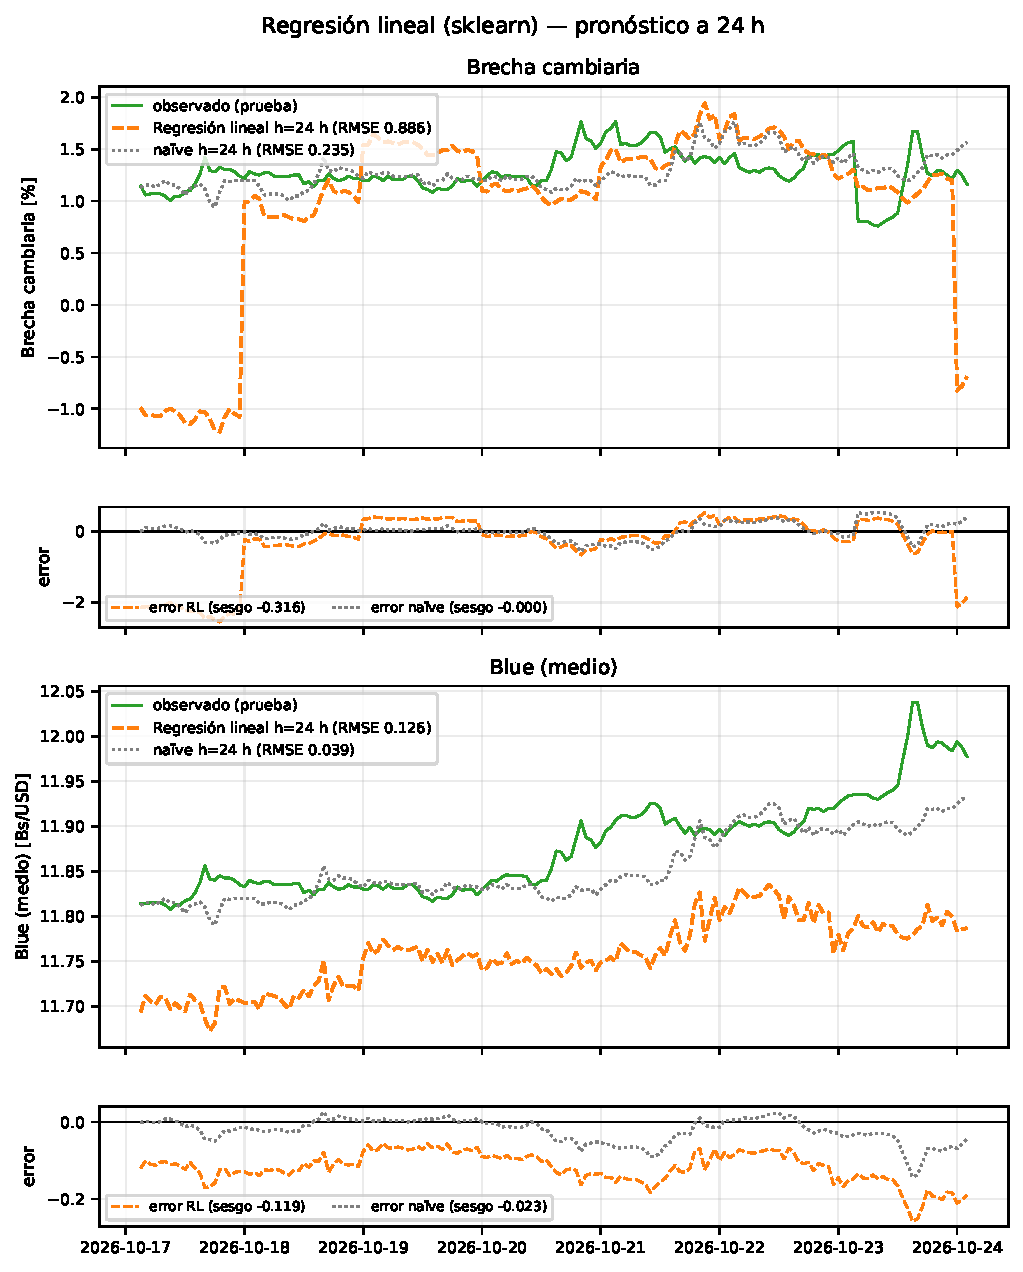
\includegraphics[width=\textwidth]{fig_rl_test.pdf}
\caption{Regresión lineal múltiple a una hora (columna izquierda) y a un día
(columna derecha) frente al observado y al naïve, en la ventana de prueba
(168~h). Cada columna muestra, para la brecha y el nivel del blue, el nivel
(arriba) y el \textbf{error} (predicción $-$ observado, abajo), con su sesgo
medio. A 24~h el error de nivel es casi constante ($-0{,}119$~Bs: predice
sistemáticamente por debajo); en la brecha el modelo se desborda en los extremos
(llega a $-2{,}5$\,pp cuando el rango observado es $0{,}8$--$1{,}8$), que es el
origen de su RMSE de $0{,}886$. A una hora el sesgo también es negativo
($-0{,}081$~Bs) y el RMSE del nivel multiplica por $10{,}6$ al del naïve.}
\label{fig:rl_test}
\end{figure}

\textbf{Lectura.} La regresión \textbf{pierde contra el naïve en los cuatro
casos}. A una hora el nivel es casi un paseo aleatorio: repetir la hora anterior
deja un error de $0{,}0077$~Bs ($0{,}07$\,\% del precio) y el modelo, con su
sesgo de nivel, llega a $0{,}0819$. A un día ambos se degradan, pero la brecha
empeora mucho más ($0{,}886$ contra $0{,}235$).

\FloatBarrier
\subsection{OLS con errores HAC (inferencia)}

El mismo diseño se reestima con \textbf{errores HAC de Newey--West} (24
rezagos, un ciclo diario), robustos a heterocedasticidad y autocorrelación: los
$\beta$ no cambian, cambia el error estándar.


\begin{table}[!ht]
\centering\small
\begin{tabular}{@{}lcccc@{}}
\toprule
Coeficiente & $\beta$ & ee HAC & $p$-valor & IC 95\% \\
\midrule
\texttt{brecha\_lag1h}  & 0{,}9899 & 0{,}0064 & $<0{,}001$ & $[0{,}9773;\,1{,}0024]$ \\
\texttt{oficial\_lag1h} & $-0{,}0263$ & 0{,}0098 & 0{,}0075 & $[-0{,}0456;\,-0{,}0070]$ \\
\bottomrule
\end{tabular}
\caption{Coeficientes significativos al 5\% (OLS + HAC sobre la brecha
horaria; $R^2$ dentro de muestra $= 0{,}9987$, $n = 4\,128$).}
\label{tab:ols_hac}
\end{table}

\begin{figure}[!ht]
\centering
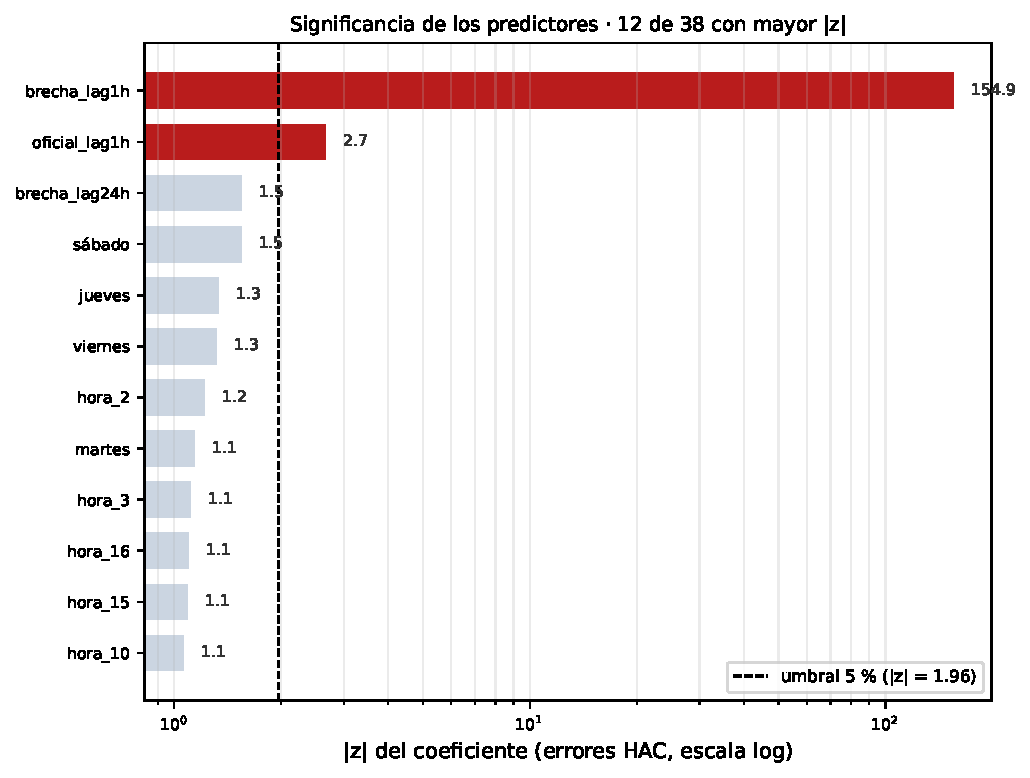
\includegraphics[width=\textwidth]{fig_hac_z.pdf}
\caption{Significancia de los coeficientes HAC: solo \texttt{brecha\_lag1h} y
\texttt{oficial\_lag1h} superan el umbral del 5\,\%; el resto tiene $|z|$
cercano a 1 (escala logarítmica).}
\label{fig:hac_z}
\end{figure}

\textbf{Lectura.} Solo dos coeficientes son significativos:
\texttt{brecha\_lag1h} ($\approx 0{,}99$, persistencia casi perfecta) y
\texttt{oficial\_lag1h} ($-0{,}026$, efecto denominador). \textbf{Ningún canal
de la Gaceta ni el volumen} resultan significativos, coherente con la
sección~4.6.

\FloatBarrier
\subsection{ARIMA}

\paragraph{Selección del orden.} El orden $(p,d,q)$ se eligió por el
\emph{criterio de información de Akaike} (AIC), calculado \textbf{solo con el
entrenamiento}, sobre una grilla con $p,q \le 2$ y $d \in \{0,1\}$
\cite{box2015timeseries}. El AIC elige ARIMA($2{,}1{,}1$) para el nivel y
ARIMA($2{,}1{,}2$) para la brecha.

La selección se repite \textbf{por horizonte}, con la ventana de entrenamiento
que corresponde a cada uno: el origen inicial de un pronóstico a $h$ pasos está
$h$ horas antes del primer objetivo, de modo que el modelo a un día no ve las
últimas 23~h de la muestra. El orden no cambia, pero el AIC sí ($-9\,305{,}0$ a
1~h y $-9\,301{,}2$ a 24~h en el nivel; $2\,926{,}5$ y $2\,931{,}4$ en la
brecha).

\begin{table}[!ht]
\centering\small
\begin{tabular}{@{}lccc@{}}
\toprule
Orden & tendencia & AIC \texttt{blue\_mid} & AIC \texttt{brecha\_pct} \\
\midrule
$(0,0,1)$ & constante & -916{,}9 & 8\,909{,}8 \\
$(0,0,2)$ & constante & -3\,121{,}2 & 7\,241{,}5 \\
$(1,0,0)$ & constante & -9\,210{,}3 & 2\,944{,}7 \\
$(1,0,1)$ & constante & -9\,299{,}4 & 2\,946{,}4 \\
$(1,0,2)$ & constante & -9\,299{,}0 & 2\,948{,}0 \\
$(2,0,0)$ & constante & -9\,291{,}8 & 2\,946{,}4 \\
$(2,0,1)$ & constante & -9\,302{,}6 & 2\,931{,}6 \\
$(2,0,2)$ & constante & -9\,297{,}5 & 2\,929{,}7 \\
$(0,1,1)$ & sin deriva & -9\,303{,}7 & 2\,948{,}2 \\
$(0,1,2)$ & sin deriva & -9\,304{,}2 & 2\,949{,}5 \\
$(1,1,0)$ & sin deriva & -9\,296{,}4 & 2\,948{,}2 \\
$(1,1,1)$ & sin deriva & -9\,304{,}6 & 2\,933{,}8 \\
$(1,1,2)$ & sin deriva & -9\,304{,}5 & 2\,931{,}0 \\
$(2,1,0)$ & sin deriva & -9\,299{,}6 & 2\,949{,}8 \\
$(2,1,1)$ & sin deriva & \textbf{-9\,305{,}0} & 2\,930{,}1 \\
$(2,1,2)$ & sin deriva & -9\,303{,}7 & \textbf{2\,926{,}5} \\
\bottomrule
\end{tabular}
\caption{Grilla completa: 16 candidatos con $p,q \le 2$ y $d \in \{0,1\}$
(constante si $d=0$, sin deriva si $d=1$). En negrita el mínimo de cada serie.
La grilla se calcula solo con entrenamiento ($n = 2\,160$) y se repite para cada
horizonte.}
\label{tab:arima_grid}
\end{table}

\begin{table}[!ht]
\centering\small
\begin{tabular}{@{}llcccc@{}}
\toprule
Target & Horizonte & RMSE & MAE & naïve & RMSE $\div$ naïve \\
\midrule
\texttt{blue\_mid} (Bs)   & 1~h  & \textbf{0{,}0074} & 0{,}0050 & 0{,}0077 & 0{,}96 \\
                          & 24~h & 0{,}0390 & 0{,}0277 & 0{,}0390 & 1{,}00 \\
\texttt{brecha\_pct} (pp) & 1~h  & 0{,}0907 & 0{,}0492 & 0{,}0910 & 1{,}00 \\
                          & 24~h & 0{,}2338 & 0{,}1786 & 0{,}2350 & 0{,}99 \\
\bottomrule
\end{tabular}
\caption{ARIMA en la ventana de prueba de 168~h, a dos horizontes, con
evaluación de origen móvil: para cada hora objetivo se pronostica desde
$t-h$ y el modelo se actualiza con los valores reales. El naïve es el último
valor observado en el origen. El orden se reselecciona por horizonte con AIC
sobre la ventana de entrenamiento correspondiente (2\,160~h): resulta
ARIMA(2,1,1) para el nivel y ARIMA(2,1,2) para la brecha en ambos casos.}
\label{tab:arima}
\end{table}

\begin{figure}[!ht]
\centering
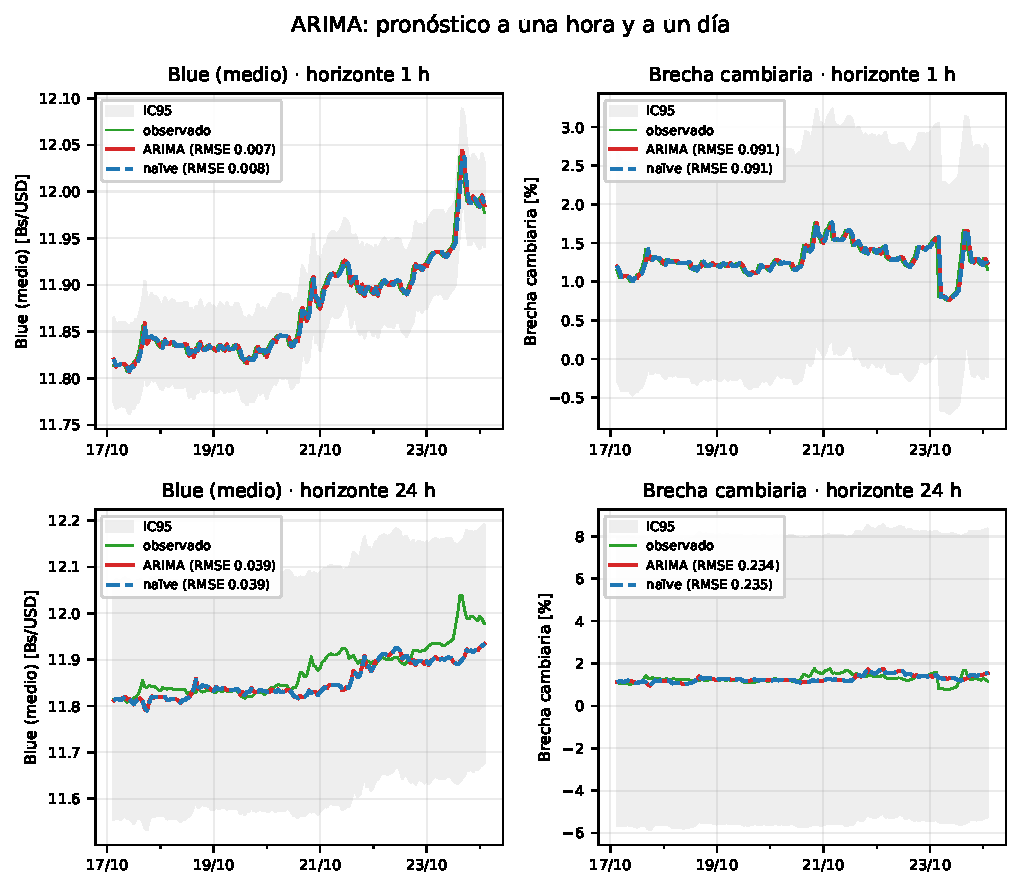
\includegraphics[width=\textwidth]{fig_arima_test.pdf}
\caption{ARIMA en la ventana de prueba (168~h) en los dos horizontes: fila
superior a una hora, fila inferior a un día. La columna izquierda es el nivel
del blue y la derecha la brecha. A una hora el pronóstico sigue de cerca al
observado y la banda es estrecha; a un día la línea del modelo se separa y la
banda se ensancha hasta cubrir casi todo el rango. En ambos casos la línea del
ARIMA anda muy cerca de la del naïve: sin deriva, el pronóstico puntual de un
paseo aleatorio es el último valor observado, y lo que aporta el modelo es la
banda de incertidumbre.}
\label{fig:arima_test}
\end{figure}

\textbf{Lectura.} El ARIMA \textbf{iguala o mejora levemente al naïve en los
cuatro casos}: a una hora reduce el RMSE del nivel un $4{,}5$\,\% y a un día las
diferencias son de una décima de punto. El valor del modelo no está en acertar
más ---el tipo de cambio horario se comporta como un paseo aleatorio
--- sino en la banda de incertidumbre.

\FloatBarrier
\subsection{Comparativa del Objetivo 1}

\begin{table}[H]
\centering\small
\begin{tabular}{@{}llccccc@{}}
\toprule
 & & & \multicolumn{2}{c}{RMSE} & \multicolumn{2}{c}{MAE} \\
\cmidrule(lr){4-5}\cmidrule(l){6-7}
Target & Horizonte & Modelo & valor & $\div$ naïve & valor & $\div$ naïve \\
\midrule
Brecha (pp)   & 1~h  & ARIMA(2{,}1{,}2) & \textbf{0{,}0907} & 1{,}00 & \textbf{0{,}0492} & 1{,}00 \\
              &      & RL múltiple      & 0{,}1175 & 1{,}29 & 0{,}0730 & 1{,}48 \\
              & 24~h & ARIMA(2{,}1{,}2) & \textbf{0{,}2338} & 0{,}99 & \textbf{0{,}1786} & 0{,}99 \\
              &      & RL múltiple      & 0{,}886  & 3{,}77 & 0{,}5504 & 3{,}05 \\
\midrule
Paralelo (Bs) & 1~h  & ARIMA(2{,}1{,}1) & \textbf{0{,}0074} & 0{,}96 & \textbf{0{,}0050} & 1{,}00 \\
              &      & RL múltiple      & 0{,}0819 & 10{,}6 & 0{,}0809 & 16{,}2 \\
              & 24~h & ARIMA(2{,}1{,}1) & \textbf{0{,}0390} & 1{,}00 & \textbf{0{,}0277} & 1{,}00 \\
              &      & RL múltiple      & 0{,}126  & 3{,}22 & 0{,}1191 & 4{,}30 \\
\bottomrule
\end{tabular}
\caption{Resumen del Objetivo 1 (ventana de prueba de 168~h), a los dos
horizontes, en RMSE y MAE. El cociente $\div$ naïve $=1$ es empate; valores
mayores indican peor desempeño. Cada modelo se compara con el naïve de su mismo
horizonte. El MAE es la magnitud que entra en el costo de operación
(sección~\ref{sec:negocio_eval}).}
\label{tab:comparativa}
\end{table}

\textbf{Lectura.} El \textbf{ARIMA domina a la regresión en los cuatro
pares} y es el único que no pierde contra su línea base: iguala al naïve a un
día ($0{,}99$--$1{,}00$) y lo mejora levemente a una hora en el nivel
($0{,}96$). La regresión múltiple, en cambio, pierde en todos los casos, con el
caso extremo del nivel a 1~h ($10{,}6\times$ en RMSE y $16{,}2\times$ en MAE).

Las dos métricas coinciden en el ordenamiento, pero el MAE matiza dos
resultados. En el nivel a una hora el ARIMA iguala al naïve en MAE ($1{,}00$)
aunque lo supere en RMSE ($0{,}96$): la ganancia está en las horas atípicas, no
en el error típico, y por eso \textbf{no se traduce en ahorro} en la
sección~\ref{sec:negocio_eval}. Y en la brecha la regresión pierde más en MAE
($1{,}48$) que en RMSE ($1{,}29$), señal de que la diferencia entre ambos se
estrecha en las horas de salto, donde el naïve acumula sus errores más grandes. El patrón es consistente con la
naturaleza de la serie: el valor de la hora anterior contiene casi toda la
información, y un modelo con 37 predictores estimados sobre seis meses no
alcanza a explotarla mejor que una regla trivial. El margen de aporte está en
la incertidumbre (sección~\ref{sec:negocio_eval}), no en el error puntual.

\FloatBarrier
\subsection{Objetivo 2 --- Publicaciones de la Gaceta y brecha}

\subsubsection{Estudio de eventos por tag}

Para cada fecha de edición de la Gaceta se toma el \texttt{blue\_mid} de las
12:00~UTC como ancla y se mide la variación porcentual a cuatro horizontes: 5
horas, 1, 3 y 5 días. Cada par (fecha, tag) es un evento; el benchmark es la
variación media de \emph{todos} los días de la serie horaria al mismo
horizonte (la deriva propia de la muestra), y el \textbf{exceso}
($\text{evento} - \text{benchmark}$) es lo interpretable como efecto de la
publicación. La serie horaria cubre 181 días (2026-04-27 $\rightarrow$
10-24), de modo que 117 de los 249 pares fecha--tag tienen datos de mercado.

\begin{table}[!ht]
\centering\small
\begin{tabular}{@{}lrrrrr@{}}
\toprule
Tag & $n$ & 5 h (pp) & 1 d (pp) & 3 d (pp) & 5 d (pp) \\
\midrule
\texttt{divisas\_control\_cambios} & 5  & $-0{,}28$ & $-0{,}31$ & $+0{,}05$ & $+0{,}95$ \\
\texttt{deuda\_externa}            & 6  & $-0{,}20$ & $+0{,}05$ & $+0{,}19$ & $+0{,}87$ \\
\texttt{comercio\_exterior}        & 12 & $-0{,}05$ & $+0{,}34$ & $+0{,}51$ & $+1{,}33$ \\
\texttt{general\_administrativo}   & 42 & $+0{,}01$ & $+0{,}26$ & $+1{,}03$ & $+1{,}21$ \\
\texttt{mineria\_energia}          & 18 & $+0{,}17$ & $+0{,}34$ & $+0{,}03$ & $+0{,}21$ \\
\texttt{impuestos}                 & 22 & $+0{,}18$ & $+0{,}37$ & $+0{,}57$ & $+1{,}05$ \\
\texttt{credito\_financiero}       & 7  & $+0{,}19$ & $+0{,}66$ & $+1{,}06$ & $+1{,}32$ \\
\texttt{fiscal\_presupuesto}       & 4  & $+0{,}50$ & $+1{,}06$ & $+3{,}83$ & $+3{,}38$ \\
\texttt{contrataciones\_estado}    & 1  & $+0{,}12$ & $+0{,}29$ & $+0{,}04$ & $+0{,}14$ \\
\bottomrule
\end{tabular}
\caption{Exceso de variación del blue sobre la línea base incondicional, por
tag y horizonte (ordenado por efecto a 5~h). También
\texttt{general\_administrativo} cruza el umbral a 3--5 días, pero es el
conjunto no cambiario: no respalda la hipótesis.}
\label{tab:eventos}
\end{table}

\textbf{Lectura.} Los tags cambiarios (\texttt{divisas\_control\_cambios},
\texttt{deuda\_externa}) son los únicos con exceso negativo a 5~h --- la
dirección que predice la hipótesis ---: \texttt{divisas} lo mantiene también a
1~día ($-0{,}31$), mientras \texttt{deuda} cambia de signo. Ninguno es
significativo con $n \geq 5$ en los horizontes cambiarios. El caso
\texttt{fiscal\_presupuesto} ($+3{,}8$~pp a 3~d) es ruido: $n=4$ y un IC95 de
$\pm7{,}2$~pp.

\subsubsection{Correlación diaria (Spearman)}

Por día se cuenta cuántas normas de cada tag se publicaron y se cruza con el
retorno diario del blue, en el mismo día ($t$) y con un día de rezago
($t{+}1$). Se usa Spearman y no Pearson porque el conteo diario es discreto y
muy sesgado hacia cero, y el retorno tiene valores atípicos; la correlación de
rangos es robusta a ambos problemas.

\textbf{Lectura.} Todas las correlaciones son débiles ($|\rho| \leq 0{,}16$):
no hay relación monótona apreciable entre la intensidad de publicación de
ningún tag y el retorno diario del blue.

\FloatBarrier
\subsection{Limitaciones}

\begin{itemize}
  \item \textbf{Una sola semana de prueba:} el RMSE depende de pocas horas
        atípicas y las diferencias entre modelos no son concluyentes con esta
        muestra.
  \item \textbf{Gaceta dispersa:} solo \textbf{23 de 179 días} tienen una norma
        con relevancia cambiaria, y por eso ningún canal resulta significativo.
\end{itemize}
